% SIAM Shared Information Template
% This is information that is shared between the main document and any
% supplement. If no supplement is required, then this information can
% be included directly in the main document.

%In this section we study the impact of parameter $\epsilon_s$ and hardware parallelism on the quality of  \acrshort{RACE} method. \Inorder to do this we first quantify the quality of the method and finally we  use this quantity to do a parameter study. The study gives insights into tuning of parameter $\epsilon_s$ based on the given matrix and required parallelism.


The \acrshort{RACE} method introduced above has a set of input parameters $\{\epsilon_s; s=0,1,\ldots\}$ which controls the assignment of number of threads to adjacent level groups. 
%For that reason a good choice is to have values close to $1$ for the initial stages and have a more relaxed constraint on the lower levels. 
To determine useful settings, we briefly analyse the interaction between these input parameters, the number of threads used and the parallel efficiency of the generated workload distribution. 

As the internal tree structure contains all information about the final workload distribution, we can use it to identify the critical path in terms of workload and correspondingly the parallel efficiency. To do so we introduce the \effRow for every node (or \levelGroup) $\acrshort{nrowsEff}(T_s(i))$  which is a measure for the absolute runtime to calculate the corresponding \levelGroup. For \levelGroups which are not further refined (leaf nodes) this value is their actual workload, i.e. the number of rows assigned to them ($\acrshort{nrowsEff}(T_0(0)) = 15$ in \cref{fig:rec_2d-7pt_tree}). For an inner node the \effRow  is the sum of the maximum workload (i.e. max. \effRow value) across each of the two colors of its leaf nodes:

\begin{align*}
\acrshort{nrowsEff}(T_s(i)) &= max(\acrshort{nrowsEff}(T_{s+1}(j) \subset T_s(i))) + max(\acrshort{nrowsEff}(T_{s+1}(j+1) \subset T_s(i)))\\
 & \text{for } j=0,2,\ldots
\end{align*}

Such definition is based on the idea that nodes at a given stage $s$ have to synchronize with each other but have to wait for their leaf nodes with the largest workload in each sweep (color) before that. Propagating this information upwards on the tree until we reach the root node constructs the critical path in terms of longest runtime taking into account single thread workloads, dependencies and synchronisation. Thus, the final value in the root node $\acrshort{nrowsEff}(T_{-1}(0))$ can be considered as the effective maximum workload of a single thread. Dividing the globally optimal workload per thread ($\frac{\acrshort{nrows}^{total}}{\acrshort{nthreads}}$) by that number gives the parallel efficiency ($\eta$) of our workload distribution: 

\begin{align*}
	\eta &= \frac{ \acrshort{nrows}^{total}} {\acrshort{nrowsEff}(T_{-1}(0)) \times \acrshort{nthreads}} 
\end{align*}
For the tree presented in \cref{fig:rec_2d-7pt_tree} the parallel efficiency is limited to $\eta=\frac{256}{44 \times 8 } = 0.73$ on eight threads, i.e. the maximum parallel speed-up is $5.8$.

\subsection{Parameter analysis and selection}

The parallel efficiency ($\eta$) as defined above can be calculated for any given matrix, number of threads $\acrshort{nthreads}$  and choice of $\{\epsilon_s; s=0,1,\ldots\}$ reflecting the RACE method's capability to generate parallelism for a problem at hand. This way we can understand the interaction between these parameters and identify useful choices for $\{\epsilon_s; s=0,1,\ldots\}$. Of course running a specific kernel such as \acrshort{SymmSpMV} on actual hardware will add other hardware and software constraints such as attainable memory bandwidth or cost of synchronisation constructs. 

In a first step we can limit the parameter space by simple corner case analysis: 
Setting all parameters close to one requests high quality load balance but may prevent our load balancing scheme from termination. In the extreme case of $\{\epsilon_s=1; s=0,1,\ldots\}$ the scheme may generate only two \levelGroups (one of each color) in each recursion, assign all threads to them and may further attempt to refine them the same way. Choosing however the values too small may introduce load imbalance by design. A range of  [0.4,0.9] for the $\epsilon_s$ values is therefore used in the following. For a basic analysis we have selected the \emph{inline} matrix (see \cref{tab:test_mtx}) as it has a rather small amount of parallelism and allows us to cover basic scenarios. In \cref{fig:inline_param_study}  we demonstrate the impact of different choices for $\epsilon_0$ and $\epsilon_1$ on the parallel efficiency for thread counts up to 100, which is a useful limit for modern CPU-based compute nodes. 
%
\begin{figure}[tbhp]
	\centering
	\subfloat[$\eta$ vs. \acrshort{nthreads} for \emph{inline} matrix ]{\label{fig:inline-a}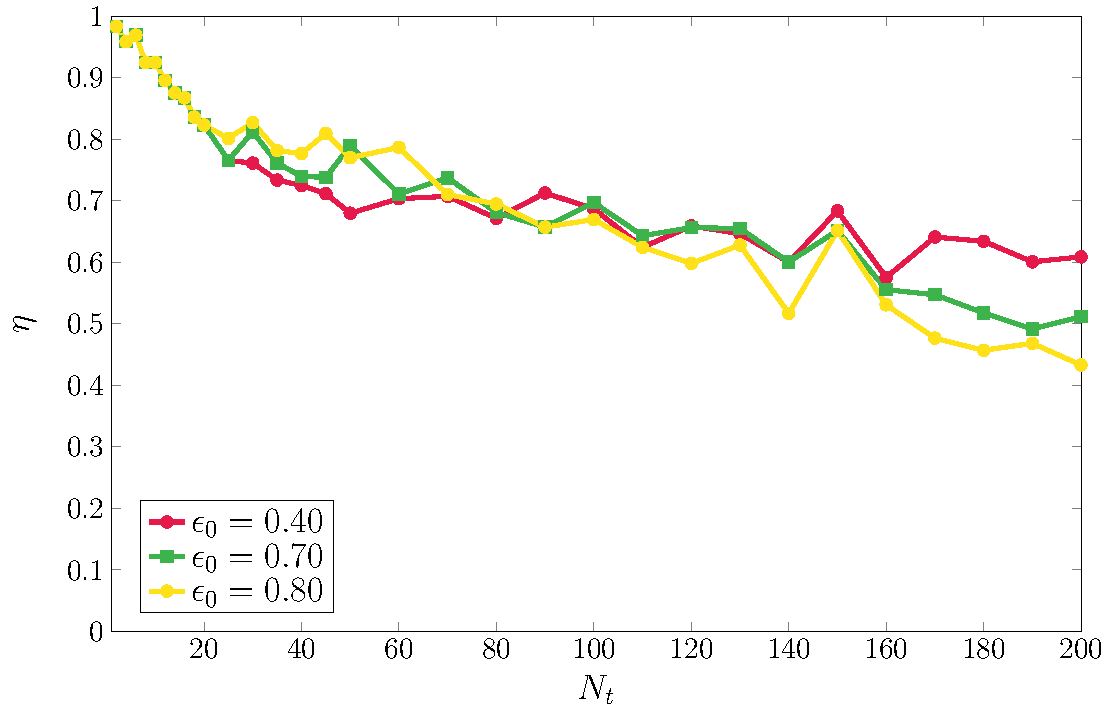
\includegraphics[width=0.45\textwidth , height=0.2\textheight]{pics/param_study/threads_vs_eff}}
	\hspace{1.5em}
	\subfloat[\acrshort{nthreads}=25]{\label{fig:inline-b}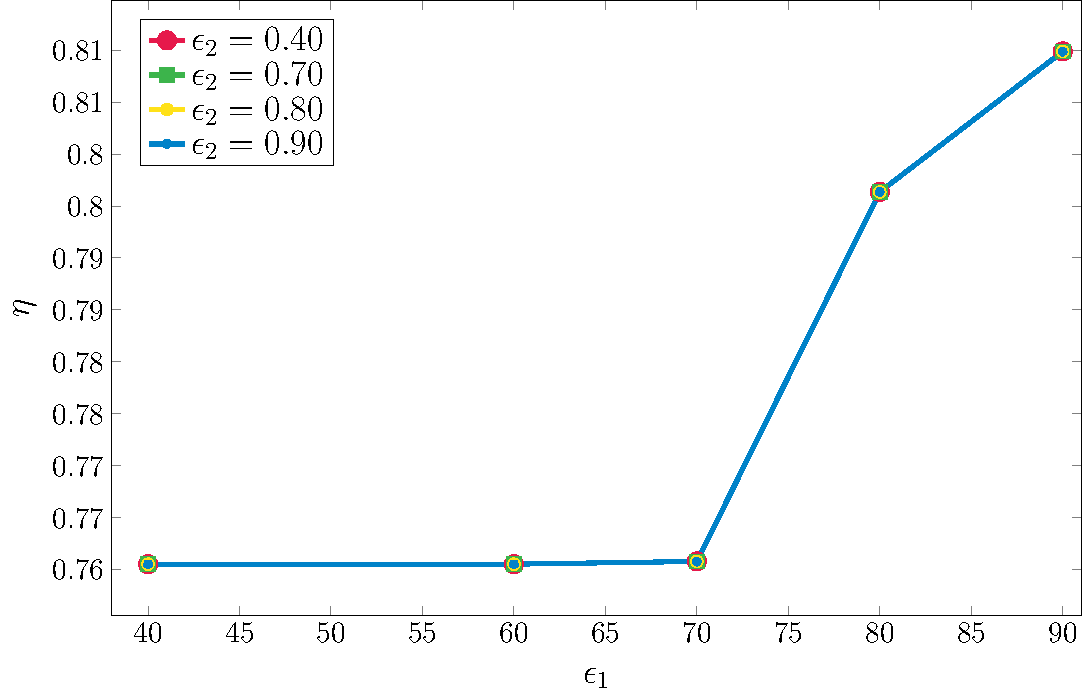
\includegraphics[width=0.45\textwidth , height=0.2\textheight]{pics/param_study/scaling_eps_1_25_threads}}
	
	\subfloat[\acrshort{nthreads}=45 ]{\label{fig:inline-c}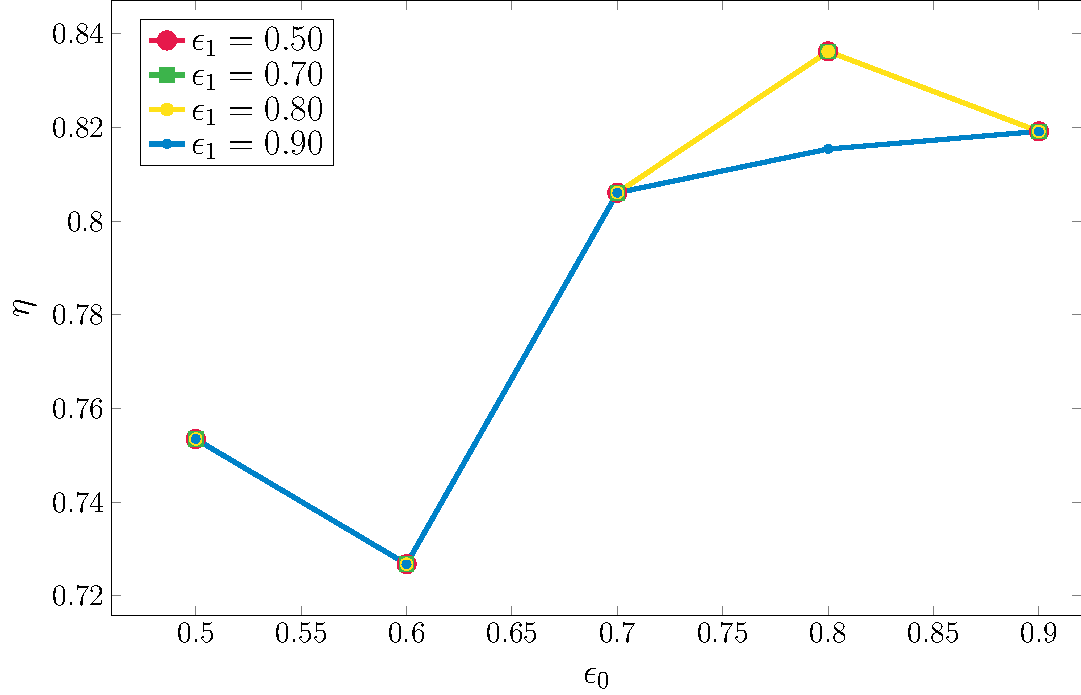
\includegraphics[width=0.45\textwidth , height=0.2\textheight]{pics/param_study/scaling_eps_1_45_threads}}
	\hspace{1.5em}
	\subfloat[\acrshort{nthreads}=100 ]{\label{fig:inline-d}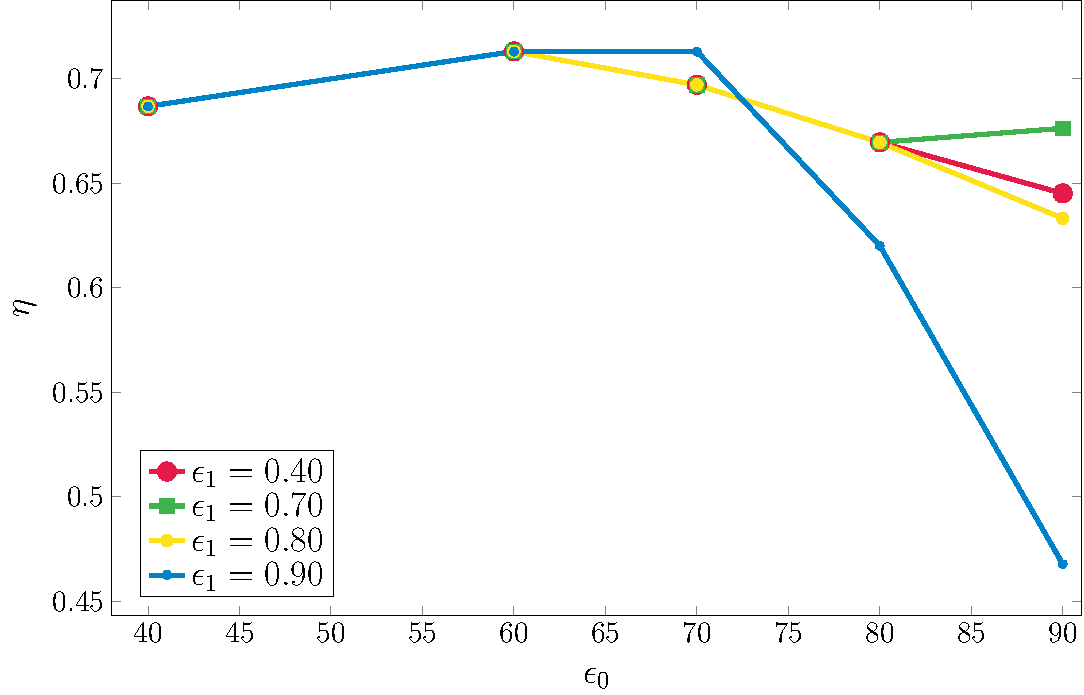
\includegraphics[width=0.45\textwidth , height=0.2\textheight]{pics/param_study/scaling_eps_1_100_threads}}
	\caption{Parameter study on \emph{inline} matrix. In \cref{fig:inline-b,fig:inline-c,fig:inline-d} each lines in the plot are iso-$\epsilon_2$ and impact of $\eta$ with respect to $\epsilon_1$ is shown. $\epsilon_s$ value if not specified is fixed to $0.4$.}
	\label{fig:inline_param_study}
\end{figure}
%
For $s > 1$ we always set the minimum value of $\epsilon_s=0.4$. The limited parallelism can be clearly observed from \cref{fig:inline-a}  with efficiency steadily decreasing with increasing thread counts. With a choice of $\epsilon_1=0.4$ there is only a minor impact of the parameter $\epsilon_0$. In \cref{fig:inline-b,fig:inline-c,fig:inline-d} the interplay between these two parameters is analysed at different thread counts in more detail. We find that up to intermediate parallelism ($\acrshort{nthreads}=50$) the exact choice has only a minor impact on the parallel efficiency (see y-axis scaling). For large levels of parallelism the interplay becomes more intricate where too large values of $epsilon_{0,1}$ may lead to larger imbalances. Based on this evaluation we choose $\epsilon_{0,1}=0.8$ and $\epsilon_s=0.4$ for $s>1$ for all the performance measurements. The quality of this choice in terms of parallel efficiency for all matrices is presented in \cref{fig:param_all_mtx_stat}. Here we plot the $\eta$ value for all matrices over a large thread count. We find that our parameter setting achieves parallel efficiencies of 80\% or higher for a substantial fraction of the matrices up to intermediate thread counts. 
   \begin{figure}[tbhp]
   	\centering
   	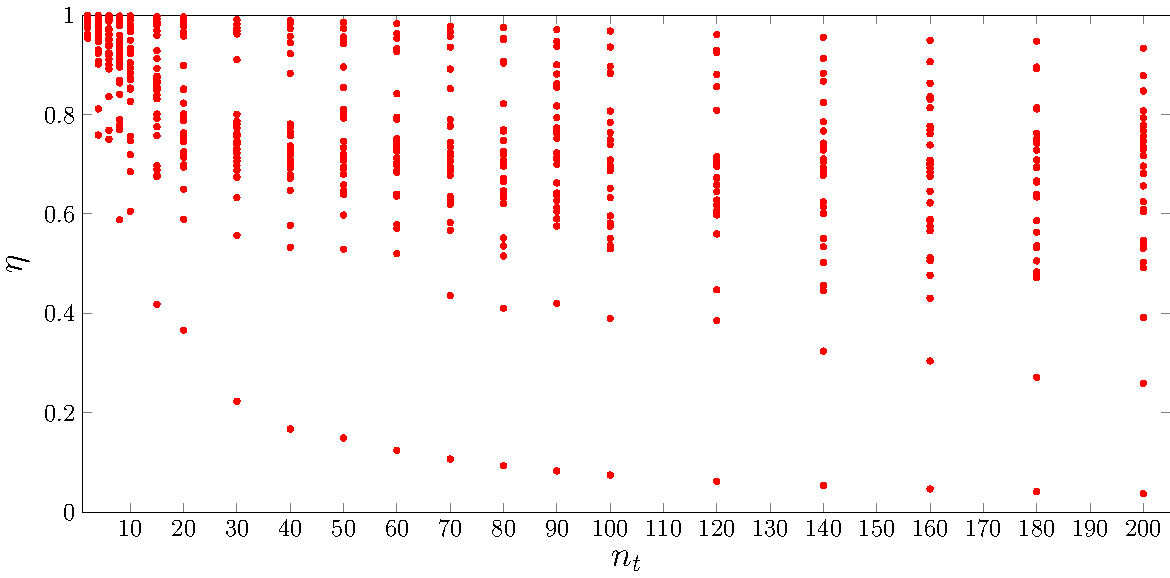
\includegraphics[height=0.19\textheight,width=0.9\textwidth]{pics/param_study/scatter_plot}
   	\caption{Scatter plot of $\eta$ vs \acrshort{nthreads} for all test matrices with $\epsilon_{0,1} = 0.8$ and $\epsilon_{s>1} = 0.4$.}
  	\label{fig:param_all_mtx_stat}
   \end{figure}
Representing the upper (lower) values in \cref{fig:param_all_mtx_stat} the best (worst) case matrix is \emph{Graphene-4096} (\emph{crankseg\_1}) exhibiting almost perfect (very) low parallel efficiencies at intermediate to high thread counts.

Finally, we evaluate the scalability of RACE using these two corner cases, the \emph{inline\_1} matrix as well as the \emph{parabolic\-fem} matrix, which is small enough to fit into the cache. 
In \cref{fig:corner_cases_param} we basically mimic a scaling test on one Skylake processor with up to 20 cores (i.e. threads) and plot the parallel efficiency as well as the maximum number of threads which can be "perfectly" used ($\eta*\acrshort{nthreads}$). 
%
\begin{figure}[tbhp]
	\centering
	\subfloat[\emph{crankseg\_1}]{\label{fig:crankseg_param}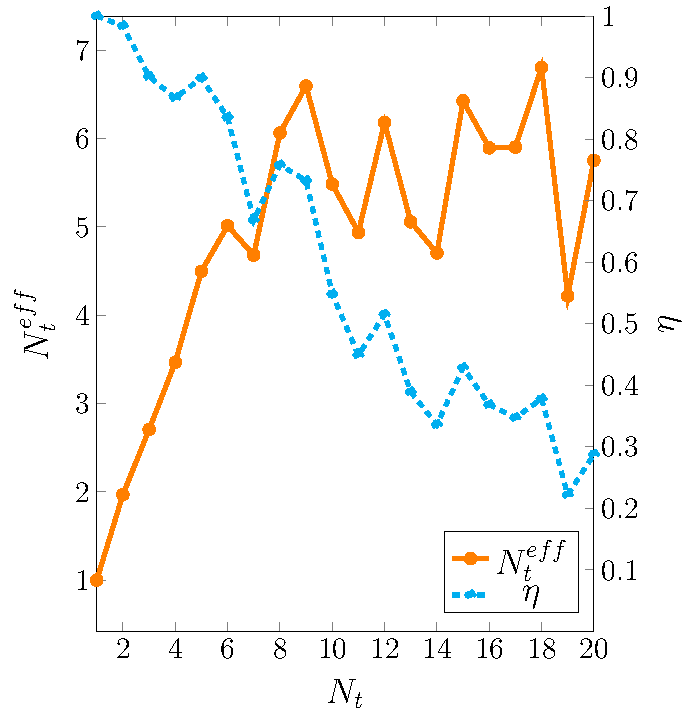
\includegraphics[width=0.23\textwidth , height=0.16\textheight]{pics/param_study/corner_cases/crankseg_1}}
	\subfloat[\emph{inline\_1}]{\label{fig:inline_param}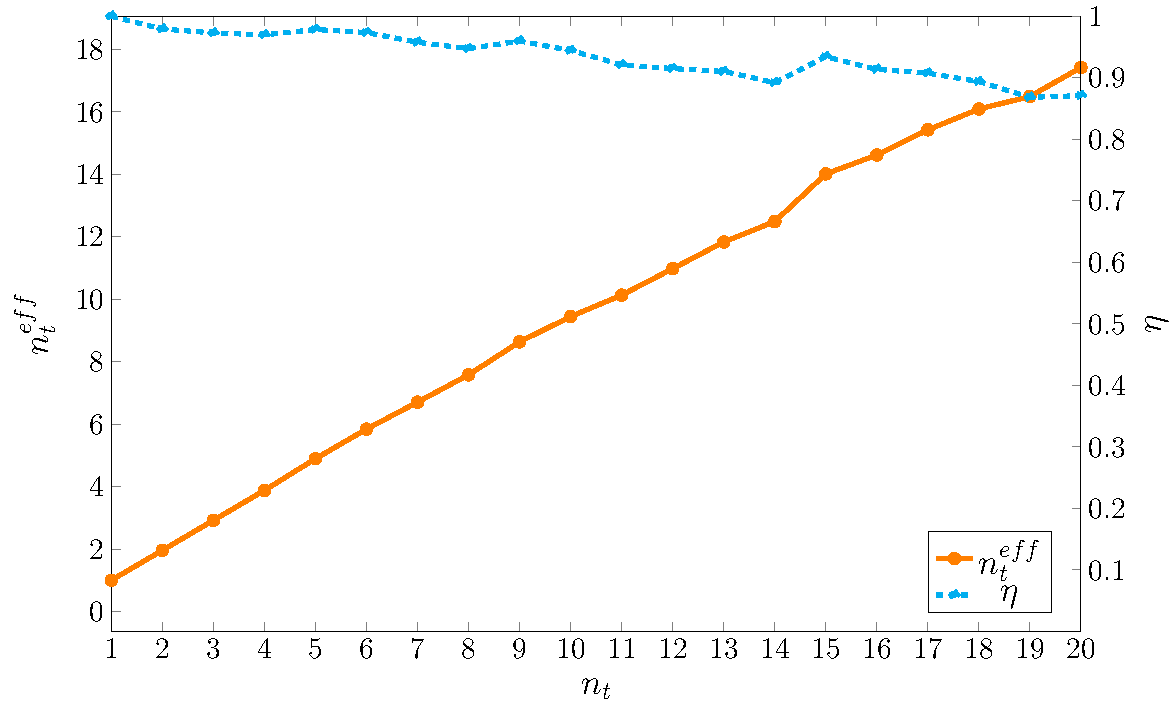
\includegraphics[width=0.23\textwidth , height=0.16\textheight]{pics/param_study/corner_cases/inline_1}}	
	\subfloat[\emph{parabolic\_fem}]{\label{fig:parabolic_fem_param}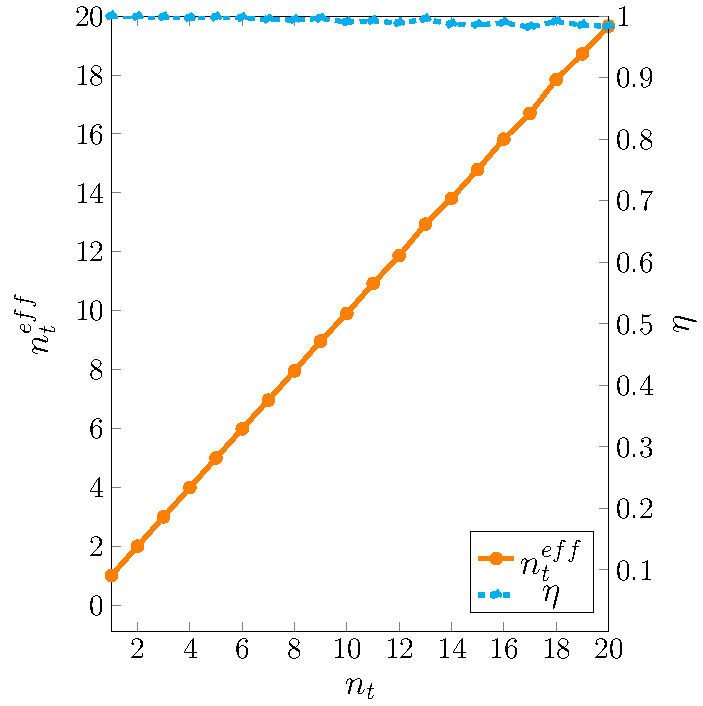
\includegraphics[width=0.23\textwidth , height=0.16\textheight]{pics/param_study/corner_cases/parabolic_fem}}
	\subfloat[\emph{Graphene-4096}]{\label{fig:Graphene-4096_param}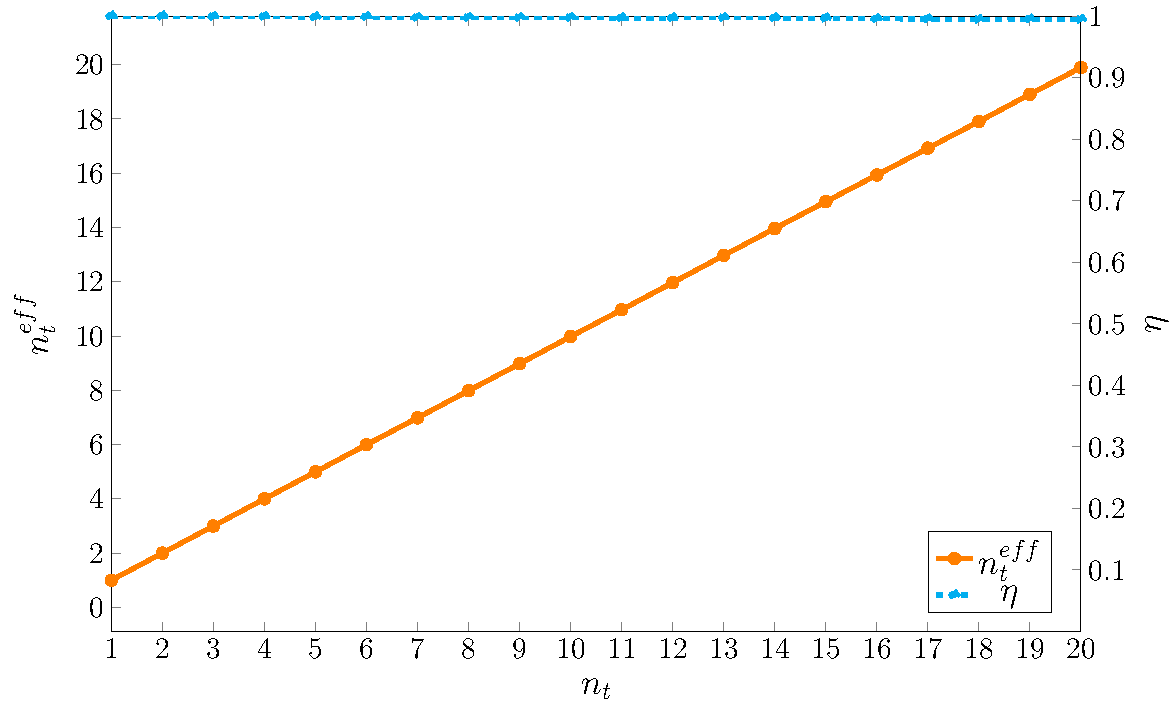
\includegraphics[width=0.23\textwidth , height=0.16\textheight]{pics/param_study/corner_cases/Graphene-4096}}	
	\caption{\acrshort{threadEff} and $\eta$ vs \acrshort{nthreads} for corner case matrices, with the same settings used in experiment runs. \acrshort{threadEff} is defined as $\eta$ * \acrshort{nthreads}.}
	\label{fig:corner_cases_param}
\end{figure}
The unfavorable structure of the \emph{crankseg\_1} matrix puts strict limits on parallelism even for low thread counts.  The combination of small matrix size, full bandwidth with a rather dense population (see ) leads to large inner levels when constructing the graph triggering strong load imbalances even for small thread counts. Searching for better $\epsilon_s$ changes the characteristic scaling but not the maximum parallelism which can be extracted. For the \emph{inline} matrix we find coherent with discussion of \cref{fig:inline_param_study} a weak but steady decrease of the parallel efficiency. The other two matrices scale very well in the range of thread counts considered. 

{\GW Will continue here...}
{\GW Probably we should continue with first measurements (fig below)}

\begin{figure}[tbhp]
	\centering
	\subfloat[\emph{crankseg\_1}]{\label{fig:crankseg_scaling}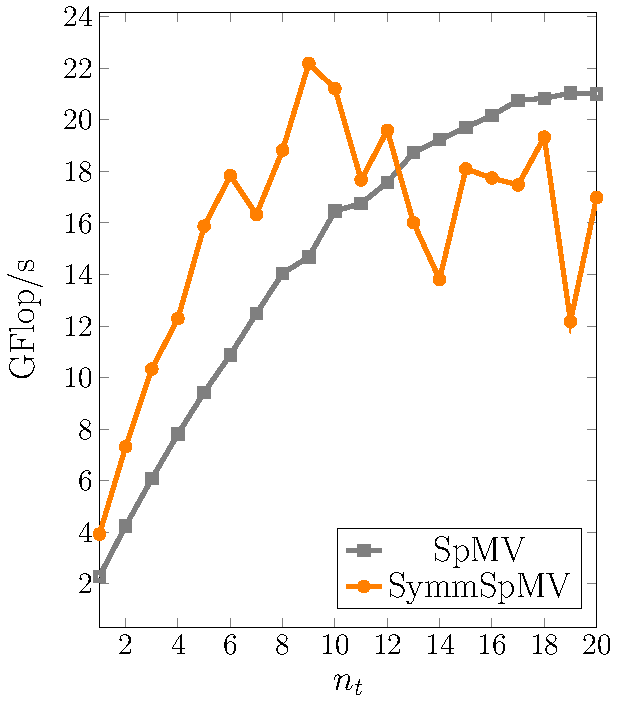
\includegraphics[width=0.23\textwidth , height=0.18\textheight]{pics/results/skx/corner_cases_scaling/plots/RCM/crankseg_1}}
	\subfloat[\emph{inline\_1}]{\label{fig:inline_scaling}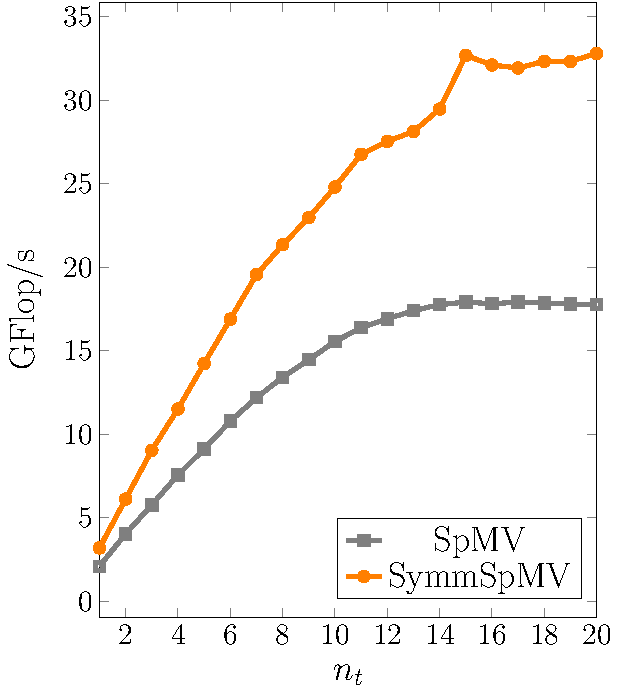
\includegraphics[width=0.23\textwidth , height=0.18\textheight]{pics/results/skx/corner_cases_scaling/plots/RCM/inline_1}}	
	\subfloat[\emph{parabolic\_fem}]{\label{fig:parabolic_fem_scaling}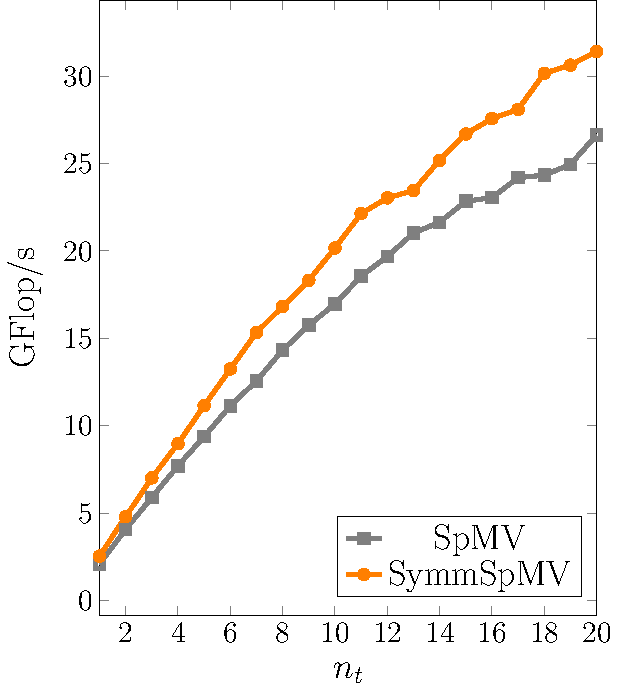
\includegraphics[width=0.23\textwidth , height=0.18\textheight]{pics/results/skx/corner_cases_scaling/plots/RCM/parabolic_fem}}
	\subfloat[\emph{Graphene-4096}]{\label{fig:Graphene-4096_scaling} 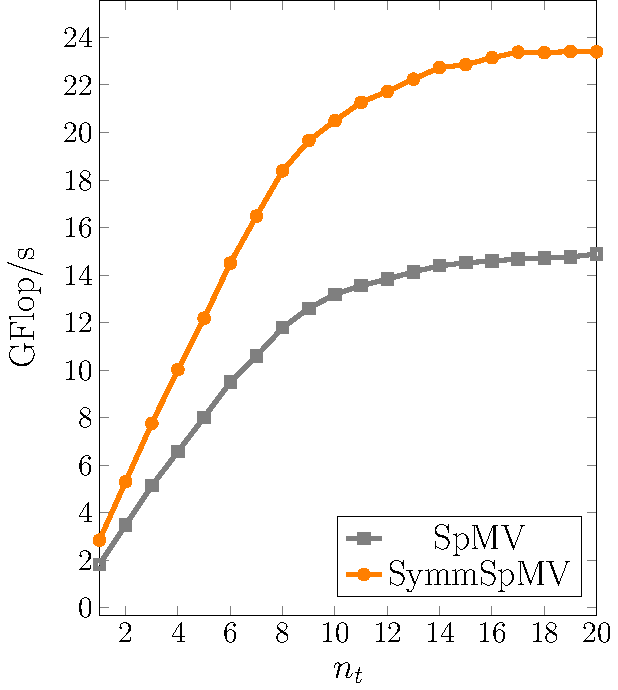
\includegraphics[width=0.23\textwidth , height=0.18\textheight]{pics/results/skx/corner_cases_scaling/plots/RCM/Graphene-4096}}	
	\caption{Scaling of \acrshort{SymmSpMV} with \acrshort{RACE} compared to \acrshort{SpMV} on one socket of \SKX architecture, for corner case matrices.}
	\label{fig:corner_cases_scaling}
\end{figure}




Quantifying quality of the method in a well-defined way is a primary and most vital step for parameter study. We do this using the concept of \effPar. From \cref{Sec:race} we saw that even though one tries to achieve parallelism exactly as that required by the hardware, in practice one might not be able to utilize this parallelism to 100 \% due to load imbalances. Therefore we use a simple calculation based on the \levelTree to determine efficiency. This takes into account load imbalances incurred from different stages of recursion. We first calculate \effRow for each of the worker leaves (leaves in finest level) in \levelTree.
The \levelGroups (leaves) in \levelTree that are not further refined form worker leaves and they are responsible for executing the rows (nodes) in their range, the work done by these leaves is therefore directly proportional to the number of rows. Hence the \effRow of these worker leaves is same as number of rows (\acrshort{nrows}), for example in case of $T_0(0)$ \effRow ( $\acrshort{nrowsEff}(T_0(0))$ = $\acrshort{nrows}(T_0(0))$ ) is 14 and $\acrshort{nrowsEff}(T_1(0) \subset T_0(4))$ is 6. After calculating the \effRow for worker leaves the information is propagated to other leaves in lower stages (up in the \levelTree) as follows: 
\begin{align*}
\acrshort{nrowsEff}(T_s(i)) &= max(\acrshort{nrowsEff}(T_{s+1}(j) \subset T_s(i))) + max(\acrshort{nrowsEff}(T_{s+1}(k) \subset T_s(i)))\\
 & \text{for } j \text{ is even and } k \text{ is odd}
\end{align*}

Such a definition for \effRow is based on the idea that a parent has to wait until the child leaf with most number of rows in each sweep (color) has finished it's work due to synchronization needed with it's siblings. This has to be handled separately for each of the two parallel sweep (colors) as there is this synchronization happening after each of the sweeps (colors). 

Once the information is propagated up the tree and as it reaches the root we have a single \effRow ($\acrshort{nrowsEff}(T_{-1})$) for the entire tree, which has taken into account load imbalance happening between all \levelGroups in all stages. The ratio of total number of rows ($\acrshort{nrows}^{total}$) in the entire matrix to that of $\acrshort{nrowsEff}(T_{-1})$ gives \effPar, denoted as \acrshort{threadEff}. Efficiency ($\eta$) of the method is then defined as ratio of  \acrshort{threadEff} to that of required hardware parallelism (\acrshort{nthreads}). 

\begin{align}
	\acrshort{threadEff} &= \frac{\acrshort{nrows}^{total}}{\acrshort{nrowsEff}(T_{-1})} \\
	\eta &= \frac{\acrshort{threadEff}}{\acrshort{nthreads}} \label{eq:eta}
\end{align}

For example in our \stex, \cref{fig:rec_2d-7pt_tree} shows \acrshort{nrowsEff} for each leaves in angular brackets and here $\acrshort{threadEff} = 5.8$ and $\eta = 0.725$. The value of $\eta = 1$ implies there is perfect load balancing which is almost impossible. In general $0 < \eta \leq 1$. This parameter $\eta$ will be used as a measure of quality in parameter study.

\subsection{Case study}
A given matrix has a fixed amount of parallelism and as the amount of required parallelism (\acrshort{nthreads}) increases load balancing degrades due to more threads per stage and imbalances between stages. The rate of degradation can however be controlled to certain extent by the tolerance $\epsilon_s$ (see \cref{eq:epsilon}) specified while choosing a \levelGroup. Typical value of $\epsilon_s$ is in range of [0.4,0.9]. Having a small $\epsilon_s$ (for example 0.4) implies we utilize the current stage `s' to maximum and do not impose high load balancing constraint, a high value on the other hand requires more balanced load from current stage `s'. 

Test matrices (see \cref{Sec:test_bed}) considered have a varying degree of parallelism, and in order to see the effect of $\eta$ and $\epsilon_s$ we choose the \emph{inline} matrix. The choice is due to the fact that this matrix has relatively small amount of parallelism and this allows us to demonstrate various effect, ranging from good to bad case scenario with small number of parallelism (\acrshort{nthreads}$ < 200$). This limited parallelism can be observed from \cref{fig:inline-a} 
where efficiency keeps on decreasing with \acrshort{nthreads} for \emph{inline} matrix. Similar behavior can be observed for \emph{crankseg\_1}, \emph{F1} and \emph{ship} matrices, of which \emph{crankseg\_1} being the worst. For majority of other test matrices one could observe that efficiency $\eta$ initially drops but then remains almost constant in the range $\eta$ = [0.50,0.80] (depending on matrix) for the entire scanned area of $1 \leq $\acrshort{nthreads}$ \leq 200$.

%\begin{figure}[tbhp]
%	\centering
%	\subfloat[$\eta$ vs \acrshort{nthreads} for \emph{inline} matrix ]{\label{fig:inline-a}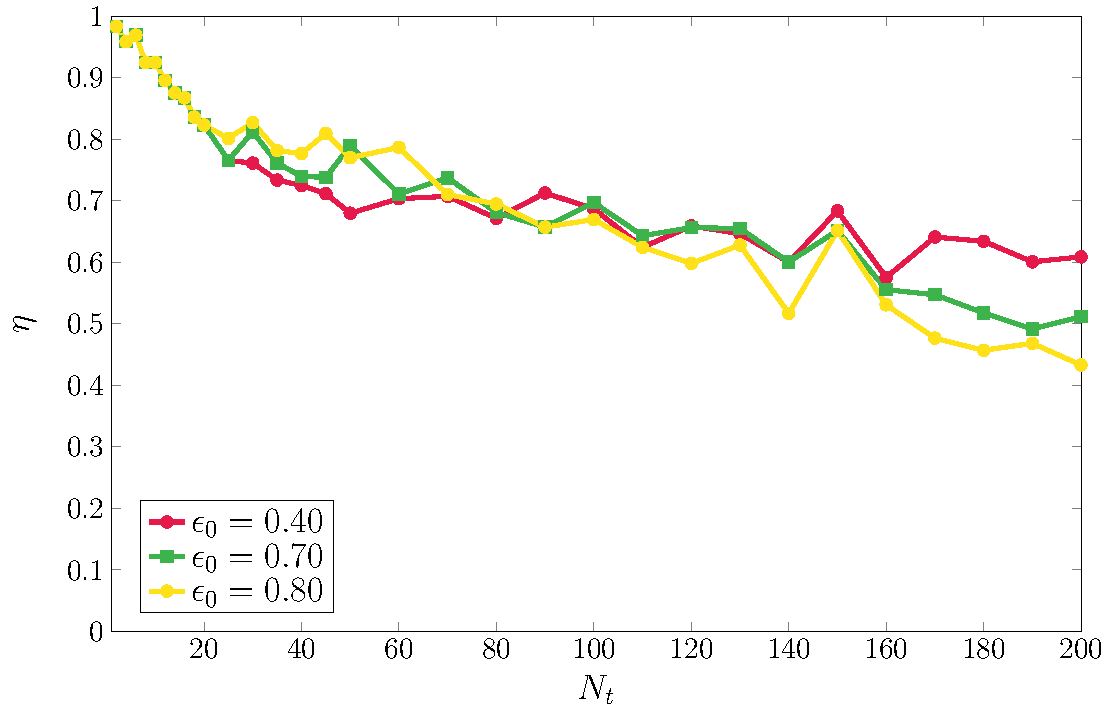
\includegraphics[width=0.45\textwidth , height=0.2\textheight]{pics/param_study/threads_vs_eff}}
%	\hspace{1.5em}
%	\subfloat[Effect of $\epsilon_0$ at low \acrshort{nthreads}, \acrshort{nthreads}=25]{\label{fig:inline-b}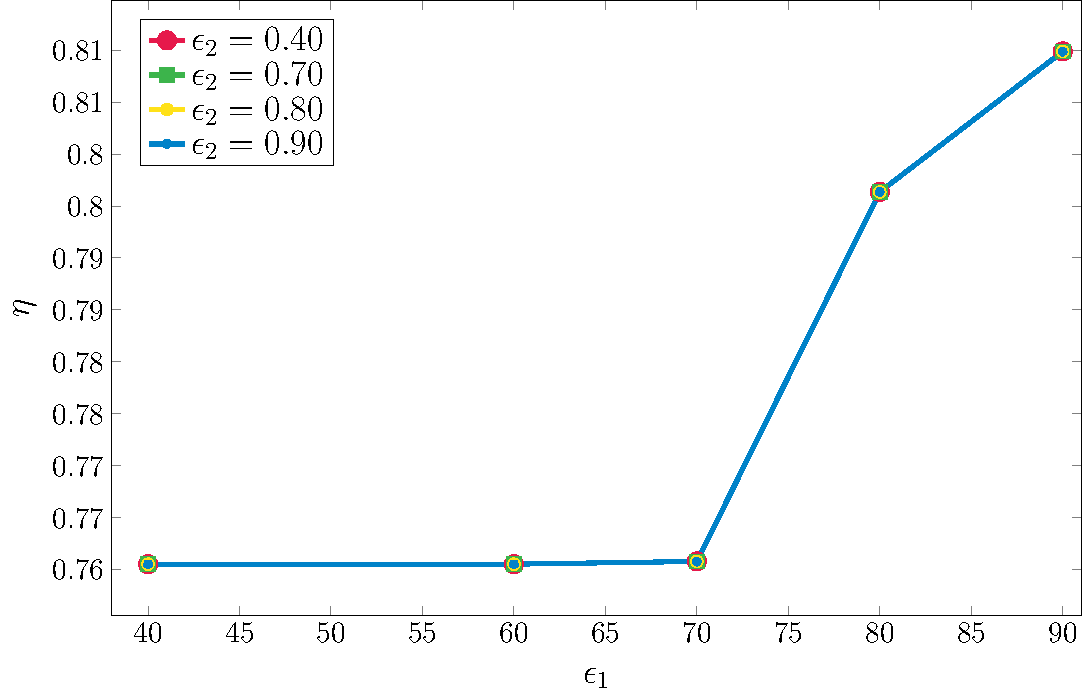
\includegraphics[width=0.45\textwidth , height=0.2\textheight]{pics/param_study/scaling_eps_1_25_threads}}
%	
%	\subfloat[Optimal $\epsilon_0$ lowered and optimal $\epsilon_1$ = 0.9, \acrshort{nthreads}=45 ]{\label{fig:inline-c}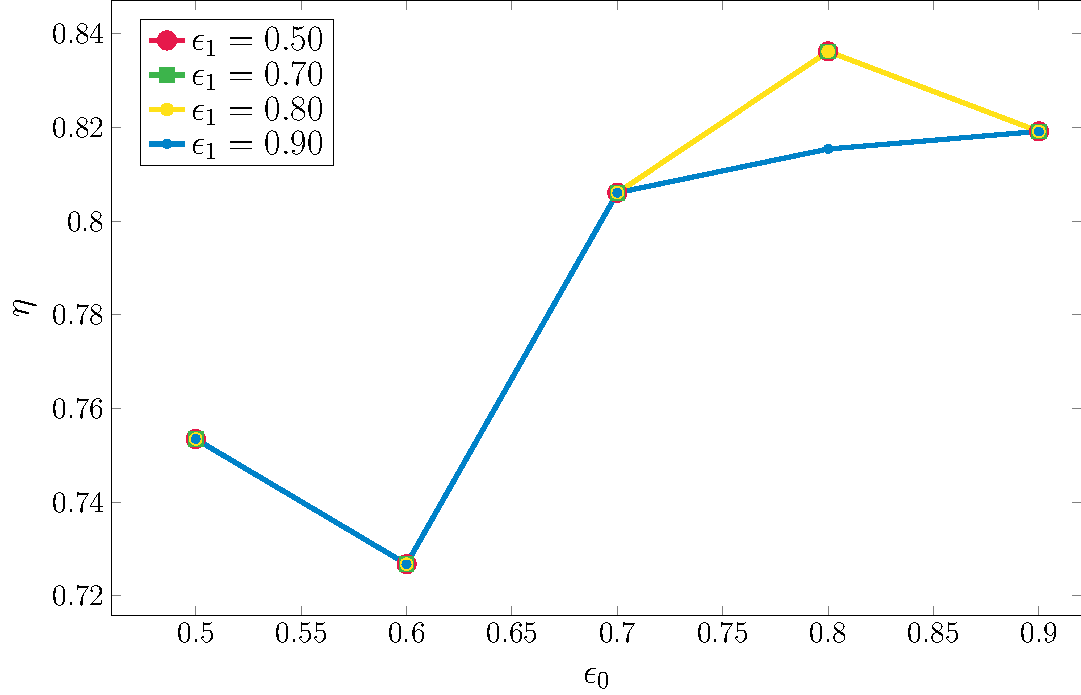
\includegraphics[width=0.45\textwidth , height=0.2\textheight]{pics/param_study/scaling_eps_1_45_threads}}
%	\hspace{1.5em}
%	\subfloat[Optimal $\epsilon_0$ lowered to 0.4 and $\epsilon_1$ to 0.7, \acrshort{nthreads}=100 ]{\label{fig:inline-d}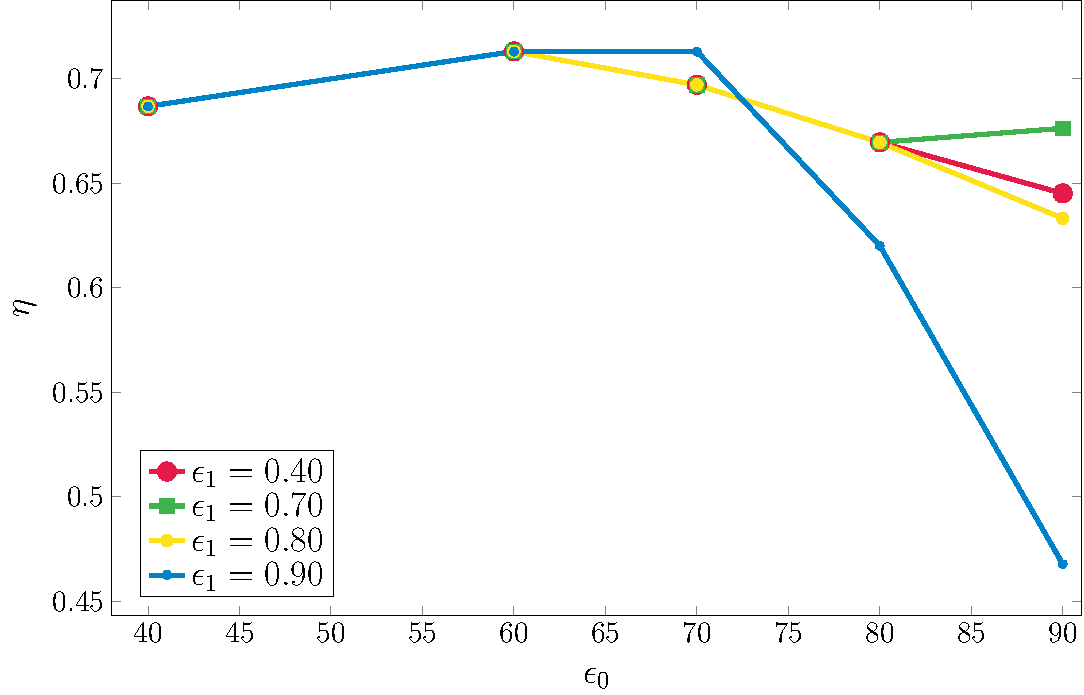
\includegraphics[width=0.45\textwidth , height=0.2\textheight]{pics/param_study/scaling_eps_1_100_threads}}
%	\caption{Parameter study on \emph{inline} matrix. In \cref{fig:inline-b,fig:inline-c,fig:inline-d} each lines in the plot are iso-$\epsilon_2$ and impact of $\eta$ with respect to $\epsilon_1$ is shown.}
%	\label{fig:inline_param_study}
%\end{figure}

At small number of threads (\acrshort{nthreads}) all matrices have high efficiency (like $\eta>0.8$). As there is a lot of parallelism in this stage compared to requirement, $\eta$ is insensitive of $\epsilon_s$. The value of \acrshort{nthreads} upto which such a behavior can be observed varies from matrix to matrix, for example \emph{inline} shows this upto \acrshort{nthreads}$\approx20$, while for matrix like \emph{Graphene} this is grater than $200$.  Further increasing \acrshort{nthreads} one could observe $\eta$ starts to vary with $\epsilon_0$. For example in case of \acrshort{nthreads}$ = 25$ one could see in \cref{fig:inline-b} maximum $\eta$ is achieved with high value of $\epsilon_0$ (0.9) due to good load balancing. But as 
\acrshort{nthreads} further increase the optimal $\epsilon_0$ starts shifting towards left (see \cref{fig:inline-c}),
 since one requires more parallelism from the current stage (s=0) and higher $\epsilon_0$ would be decremental since it would require the \levelTree to go more deep and hence load imbalances in next stages will get multiplied. $\epsilon_1$ which till now didn't effect much starts to influence slowly as \acrshort{nthreads} increments again, for example in case of \emph{inline} till $\acrshort{nthreads}=90$ $\epsilon_1=0.9$ was optimal, but then the optimal $\epsilon_1$ reduces and reaches $0.7$ at \acrshort{nthreads}$=190$ as seen in \cref{fig:inline-d}. $\eta$ would start to get affected by $\epsilon_s$ of next stages in similar manner with increase of \acrshort{nthreads}.
 
Behavior of other matrices in the test bed follow similar pattern, but \acrshort{nthreads} at which different phases occur varies from matrix to matrix.  \Cref{fig:param_all_mtx_stat} gives a broad overview of the efficiency ($\eta$) behavior of entire test matrices using scatter plot. Each point at a specific \acrshort{nthreads} represents efficiency ($\eta$) of a matrix. Majority of test matrices having an initial drop in $\eta$ and then remaining constant is reflected in the statistical plot. The lowest points in the plot correspond to \emph{crankseg\_1} matrix, here we achieve only a mere parallelism of eight at maximum (\acrshort{threadEff} = 8), while the upper points correspond to matrix having highest parallelism namely \emph{Graphene} matrix.

In practice for a given matrix it's difficult to precisely determine the optimal rate of decrease in $\epsilon_s$ without parameter search, and therefore selecting proper $\epsilon_s$ for given \acrshort{nthreads} can be challenging. One idea is to see total levels (\acrshort{totalLvl}) and distribution of non-zeros (\acrshort{nnz}) in different levels of current stage `s' and heuristically determine $\epsilon_s$ based on the pressure of parallelism from stage `s'. This is not currently done and is part of our future work. As a rule of thump an $\epsilon_{0,1} = 0.8$ and $\epsilon_{s>1} = 0.4$ is sufficient for most matrices on current architectures, therefore currently for experiments we set these $\epsilon_s$ values for all matrices.

 In \cref{fig:corner_cases_param} we have plotted \acrshort{threadEff} and $\eta$ vs \acrshort{nthreads} for corner case matrices with the settings used in experiment runs. Here we set $\epsilon_{0,1}=0.8$ and use \acrfull{RCM} in the \emph{level construction} stage (\cref{subsec:LEVEL_CONST}). Big fluctuation in \emph{crankseg\_1} is due to the fact that we set high load balancing requirement (high $\epsilon_s$ factor) and as seen in the example of \emph{inline\_1} matrix this is not optimal when we reach the limit of parallelism. The theoretical estimates obtained in \cref{fig:corner_cases_param} will be directly used to compare with experiment runs in the next section (\cref{Sec:expt}).

